\documentclass{beamer}
\usepackage{graphicx}

\usepackage[utf8]{inputenc}
\usepackage[T1]{fontenc} 

\usetheme[hideallsubsections]{PaloAlto}

%\usepackage{tikz}
\usepackage{verbatim}
\usepackage{tabularx}
\usepackage{array}

% vertically centering in tables when X
\renewcommand{\tabularxcolumn}[1]{>{\small}m{#1}}
\usepackage{makecell}
\usepackage{color}
\usepackage{diagbox}

\usepackage[english]{babel}
\usepackage{lmodern} 


% \setbeamertemplate{sections in toc}[sections numbered]
% \usetikzlibrary{arrows,shadows,shapes,backgrounds,positioning}
% \beamertemplatetransparentcovered

% insert page number in Beamer Navigation Bars
\addtobeamertemplate{navigation symbols}{}{%
    \usebeamerfont{footline}%
    \usebeamercolor[fg]{footline}%
    \hspace{1em}%
    \insertframenumber/\inserttotalframenumber
}

% set head height
\makeatletter
\setlength{\beamer@headheight}{0.7cm}
\makeatother


\title[]{Communautés et contributions aux logiciels libres} 
\author{Rémi Boulle}
\date{}       
\institute{}        

\begin{document}

% section titles in a special slide
\AtBeginSection[]{
  \begin{frame}
  \vfill
  \centering
  \begin{beamercolorbox}[sep=8pt,center,shadow=true,rounded=true]{title}
    \usebeamerfont{title}\insertsectionhead\par%
  \end{beamercolorbox}
  \vfill
  \end{frame}
}

%%%%%%%%%%%%%%%%
% Title
%%%%%%%%%%%%%%%%

\begin{frame}
  \titlepage
\end{frame}


\section{Économie du libre}

\begin{frame}{Vendre ce qui est gratuit ??}
  \begin{block}{François Élie :}
 "Un logiciel libre est gratuit une fois qu'il a été payé"
\end{block}

\begin{alertblock}{Modèles économiques}
  Modèle de rente vs modèle de service.
\end{alertblock}
\end{frame}

\begin{frame}{Modèles économiques}
  \begin{itemize}
  \item Éditeur : \only<2>{\textbf{Bluemind, Adacore, Kélis, Centréon...}}
  \item Distributeur à valeur ajoutée  \only<2>{\textbf{Canonical, Redhat...}}
  \item Fournisseur d'applications hébergées (SaaS, Cloud)  \only<2>{\textbf{IBM avec Openstack, automattic...}}
  \item Services à valeur ajoutée (ENL)  \only<2>{\textbf{Makina Corpus, Linagora...}}
  \item Intégrateur hybride (produit+service)  \only<2>{\textbf{Logilab, Smile, Alter way...}}
  \end{itemize}
  
\end{frame}

\section{Contributions}

\begin{frame}{Typologie des contributions}

  \begin{itemize}
  \item Faire partie d'une communauté en étant désintéressé
  \item Monter en compétences (CV)
  \item contributions tactiques (pour soi, ses propres outils...)
  \item contributions stratégiques (pour le projet en lui-même)
  \end{itemize}

  Déséquilibre et \textit{Tragédie des communs...}

  
\end{frame}

\begin{frame}{Des projets libres}
  Trois types de projets libres :
  \begin{itemize}
  \item Vitrine "libre" d'une entreprise sur github (pas de contributions attendues)
  \item Projets pseudo-ouverts (bénéfice direct pour le propriétaire)
  \item De vrais \textbf{communs} entre pairs à droits égaux
  \end{itemize}
\end{frame}

\section{Exemples de communauté}


\setbeamertemplate{background canvas}{\hspace{1.6cm}
\includegraphics[width=\textwidth]{images/heartbleed.png}}
\begin{frame}[plain]%{OpenSSL}
%  
\end{frame}
\setbeamertemplate{background canvas}{}

\setbeamertemplate{background canvas}{\centering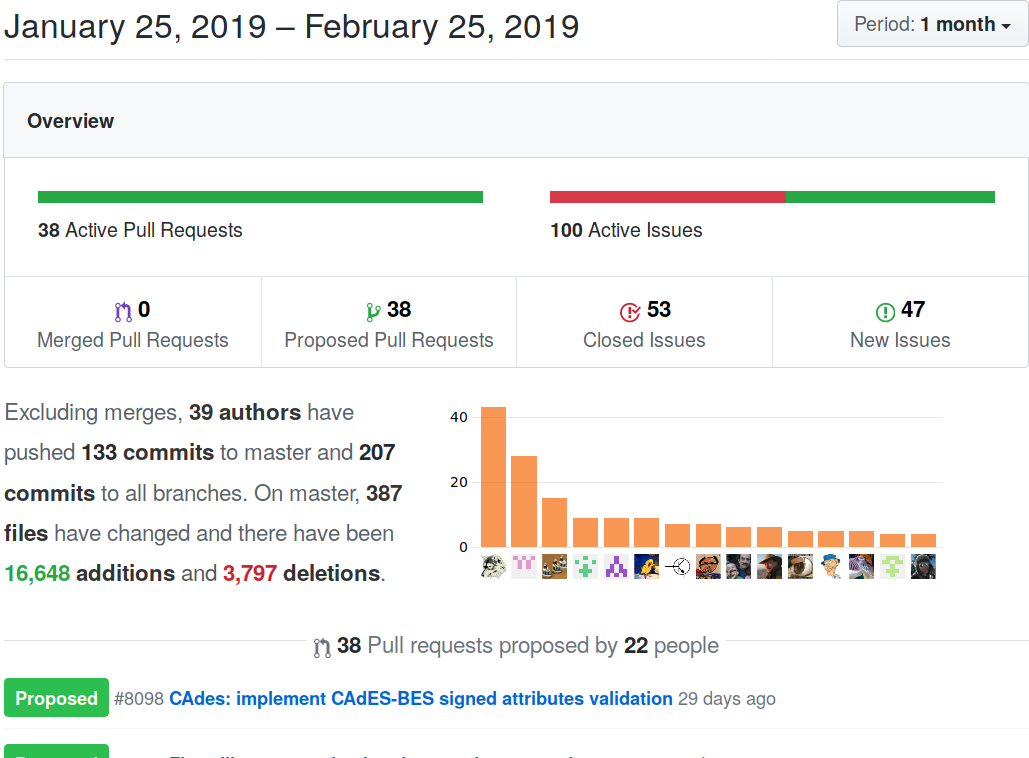
\includegraphics[width=\paperwidth]{images/openssl.png}}
\begin{frame}[plain]%{OpenSSL}
%  
\end{frame}
\setbeamertemplate{background canvas}{}

\begin{frame}{Firefox}
  \url{https://www.openhub.net/p/firefox}
\end{frame}

\begin{frame}{Django}

  \begin{block}{First steps}
    \textit{The code that you write belongs to you or your employer. If your contribution is more than one or two lines of code, you need to sign the CLA.}
  \end{block}

  Plus d'infos sur : \url{https://docs.djangoproject.com/en/dev/internals/contributing/}
\end{frame}


\begin{frame}{LibreOffice}
  Voir \url{https://dashboard.documentfoundation.org}
\end{frame}

\section{Contribuer/Utiliser}

\begin{frame}{Contexte}

  \begin{block}{Contribuer/utiliser}
    Le libre est maintenant partout...
  \end{block}
  Deux cas :
  \begin{itemize}
  \item Vous êtes salarié d'une entreprise en informatique :
    \begin{itemize}
    \item Y-a-t-il une gouvernance autour du libre ? (risques techniques, juridiques et financiers)
    \item Y-a-t-il une politique/charte qui encadre/favorise la contribution ?
    \item Posez la question, réponse par écrit.
    \end{itemize}
  \item Autres cas...
  \end{itemize}
  
\end{frame}

\end{document}

Image bug d'OpenSSL (heartbleed) : https://commons.wikimedia.org/wiki/File:Heartbleed.svg par Leena Snidate / Codenomicon (licence CC0).

%%% Local Variables:
%%% mode: latex
%%% TeX-master: t
%%% End:
